\section{Object management functions}


\subsection{xlpType}

\begin{xlpfunctitle}{xlpType}

\begin{xlpfunc}{Parameters}
\begin{tabular}{p{3.5cm}cl}
\textbf{scalar}& : & scalar code \\
\textbf{trigger}& : & trigger 
\end{tabular}
\end{xlpfunc}


\begin{xlpfunc}{Returns}
A cell matrix of dimension (1, 1)
\end{xlpfunc}

\begin{xlpfunc}{Description}
Return the type of scalar. 
\end{xlpfunc}
\end{xlpfunctitle}


\subsection{xlpListAllObjects}

\begin{xlpfunctitle}{xlpListAllObjects}

\begin{xlpfunc}{Parameters}
\begin{tabular}{p{3.5cm}cl}
\textbf{transpose}& : & transpose ouput \\
\textbf{trigger}& : & trigger 
\end{tabular}
\end{xlpfunc}

\begin{xlpfunc}{Returns}
A cell matrix of dimension (2, n)
\end{xlpfunc}

\begin{xlpfunc}{Description}
Return all the python objects. The first column is the object name, the second column is the type of the object 

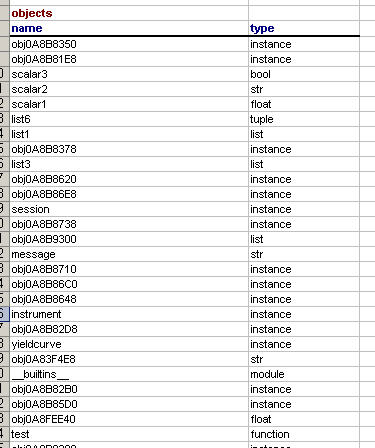
\includegraphics[width=8cm]{images/objects.jpg}
\end{xlpfunc}
\end{xlpfunctitle}


\subsection{xlpDeleteAllObjects}

\begin{xlpfunctitle}{xlpDeleteAllObjects}

\begin{xlpfunc}{Parameters}
\begin{tabular}{p{3.5cm}cl}
\textbf{trigger}& : & trigger 
\end{tabular}
\end{xlpfunc}


\begin{xlpfunc}{Returns}
Character string equal to "success" in case of no error.
\end{xlpfunc}

\begin{xlpfunc}{Description}
Delete all objects.
\end{xlpfunc}
\end{xlpfunctitle}

\subsection{xlpDeleteObject}

\begin{xlpfunctitle}{xlpDeleteObject}

\begin{xlpfunc}{Parameters}
\begin{tabular}{p{3.5cm}cl}
\textbf{scalar}& : & scalar code \\
\textbf{trigger}& : & trigger 
\end{tabular}
\end{xlpfunc}


\begin{xlpfunc}{Returns}
Character string equal to "sucess" in case of no error.
\end{xlpfunc}

\begin{xlpfunc}{Description}
Delete object defined by scalar.
\end{xlpfunc}

\end{xlpfunctitle}

\subsection{xlpListAllAttr}

\begin{xlpfunctitle}{xlpListAllAttr}

\begin{xlpfunc}{Parameters}
\begin{tabular}{p{3.5cm}cl}
\textbf{scalar}& : & scalar code \\
\textbf{transpose}& : & transpose of output \\
\textbf{trigger}& : & trigger 
\end{tabular}
\end{xlpfunc}


\begin{xlpfunc}{Returns}
Cell matrix of dimension (5, n) where n is the number of attributes.
\end{xlpfunc}

\begin{xlpfunc}{Description}
List all the attributes of the scalar code:
\begin{itemize}
\item the column 1 is the name of the attribute 
\item the column 2 is the type
\item the column 3 is the minimum number of arguments
\item the column 4 say if the attribute is callable (a function)
\item the column 5 say if the attribute can accept a variable number of arguments (for function only).
\end{itemize}

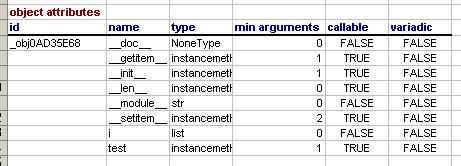
\includegraphics[width=11cm]{images/listallattr.jpg}
\end{xlpfunc}
\end{xlpfunctitle}

\subsection{xlpAttrInfos}

\begin{xlpfunctitle}{xlpAttrInfos}

\begin{xlpfunc}{Parameters}
\begin{tabular}{p{3.5cm}cl}
\textbf{scalar}& : & scalar code \\
\textbf{attr}& : & attribute name (character string) \\
\textbf{transpose}& : & transpose of output \\
\textbf{trigger}& : & trigger 
\end{tabular}
\end{xlpfunc}


\begin{xlpfunc}{Returns}
Cell matrix of dimension (4, 1).
\end{xlpfunc}

\begin{xlpfunc}{Description}
List all the attributes of the scalar code:
\begin{itemize}
\item the column 1 is the type
\item the column 2 is the minimum number of arguments
\item the column 3 say if the attribute is callable (a function)
\item the column 4 say if the attribute can accept a variable number of arguments (for function only).
\end{itemize}
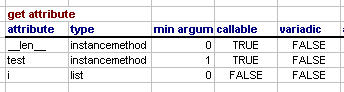
\includegraphics[width=11cm]{images/getattribute.jpg}
\end{xlpfunc}

\end{xlpfunctitle}